\documentclass{beamer}
\let\vec\mathbf
\mode<presentation>
\usepackage{amsmath}
\usepackage{amssymb}
%\usepackage{advdate}
\usepackage{adjustbox}
%\usepackage{subcaption}
\usepackage{enumitem}
\usepackage{multicol}
\usepackage{mathtools}
\usepackage{listings}
\usepackage{url}
\usepackage{gensymb}
\usetheme{Boadilla}
\usecolortheme{lily}
\setbeamertemplate{footline}
{
  \leavevmode%
  \hbox{%
  \begin{beamercolorbox}[wd=\paperwidth,ht=2.25ex,dp=1ex,right]{author in head/foot}%
    \insertframenumber{} / \inserttotalframenumber\hspace*{2ex} 
  \end{beamercolorbox}}%
  \vskip0pt%
}
\setbeamertemplate{navigation symbols}{}
\providecommand{\nCr}[2]{\,^{#1}C_{#2}} % nCr
\providecommand{\nPr}[2]{\,^{#1}P_{#2}} % nPr
\providecommand{\mbf}{\mathbf}
\providecommand{\pr}[1]{\ensuremath{\Pr\left(#1\right)}}
\providecommand{\qfunc}[1]{\ensuremath{Q\left(#1\right)}}
\providecommand{\sbrak}[1]{\ensuremath{{}\left[#1\right]}}
\providecommand{\lsbrak}[1]{\ensuremath{{}\left[#1\right.}}
\providecommand{\rsbrak}[1]{\ensuremath{{}\left.#1\right]}}
\providecommand{\brak}[1]{\ensuremath{\left(#1\right)}}
\providecommand{\lbrak}[1]{\ensuremath{\left(#1\right.}}
\providecommand{\rbrak}[1]{\ensuremath{\left.#1\right)}}
\providecommand{\cbrak}[1]{\ensuremath{\left\{#1\right\}}}
\providecommand{\lcbrak}[1]{\ensuremath{\left\{#1\right.}}
\providecommand{\rcbrak}[1]{\ensuremath{\left.#1\right\}}}
\theoremstyle{remark}
\newtheorem{rem}{Remark}
\newcommand{\sgn}{\mathop{\mathrm{sgn}}}

\newcommand{\abs}[1]{\left|#1\right|}

\providecommand{\res}[1]{\Res\displaylimits_{#1}} 
\providecommand{\norm}[1]{\lVert#1\rVert}
\providecommand{\mtx}[1]{\mathbf{#1}}

\providecommand{\fourier}{\overset{\mathcal{F}}{ \rightleftharpoons}}
%\providecommand{\hilbert}{\overset{\mathcal{H}}{ \rightleftharpoons}}
\providecommand{\system}{\overset{\mathcal{H}}{ \longleftrightarrow}}
 %\newcommand{\solution}[2]{\textbf{Solution:}{#1}}
%\newcommand{\solution}{\noindent \textbf{Solution: }}
\providecommand{\dec}[2]{\ensuremath{\overset{#1}{\underset{#2}{\gtrless}}}}
\newcommand{\myvec}[1]{\ensuremath{\begin{pmatrix}#1\end{pmatrix}}}

\title{Matrices in Geometry - 10.5.3}
\author{EE25BTECH11035 Kushal B N}
\date{}

\begin{document}

\maketitle

\section{Problem Statement}
\begin{frame}
\frametitle{Problem Statement}
Draw a pair of tangents to a circle of radius $5cm$ which are inclined to each other at an angle of $60\degree$.
\end{frame}

\section{Solution}
\begin{frame}{Solution}
Let the center be the origin. Then the circle with radius 5 $5cm$ iw
\begin{equation}
    \vec{C} : \vec{x}^{\top}\vec{V}\vec{x} + 2\vec{u}^{\top}\vec{x} + f = 0
\end{equation}
where,
\begin{equation}
    \vec{V} = \myvec{1&0\\0&1} \text{ , } \vec{u} = \myvec{0\\0} \text{ , } f = -25
\end{equation}

Let the tangents be drawn from an external point $\vec{h}$.
Line segment from $O$ to $h$ bisects the angle between the tangents and it forms two right angled triangles.
So that, we have
\begin{equation}
    \sin{\frac{60 \degree}{2}} = \frac{r}{\norm{\vec{h}}} = \frac{5}{\norm{\vec{h}}}
\end{equation}

\begin{equation}
    \implies \norm{\vec{h}} = \frac{5}{\sin{30 \degree}} = 10
\end{equation}
\end{frame}

\begin{frame}{Solution}
So the point $h$ should be at a distance of $10cm$ from the origin(centre).
Let the point be
\begin{equation}
    \vec{h} = \myvec{10\\0}
\end{equation}

Calculating the matrix $\Sigma$
\begin{equation}
    \Sigma = (\vec{V}\vec{h} + \vec{u})(\vec{V}\vec{h} + \vec{u})^{\top} - g(\vec{h})\vec{V}
\end{equation}

\begin{equation}
    g(\vec{h}) = \vec{h}^{\top}\vec{V}\vec{h} + 2\vec{u}^{\top}\vec{h} + f = \norm{\vec{h}}^2 + f = 100 - 25 = 75
\end{equation}

\begin{equation}
    \Sigma = \vec{h}\vec{h}^{\top} - g(\vec{h})\vec{V} = \myvec{10\\0}\myvec{10&0} - 75\myvec{1&0\\0&1}
\end{equation}

\begin{equation}
    \implies \Sigma = \myvec{25&0\\0&-75}
\end{equation}
\end{frame}

\begin{frame}{Solution}
The eigen values of the matrix $\Sigma$ are 
\begin{equation}
    \lambda_1 = 25
\end{equation}

\begin{equation}
    \lambda_2 = -75
\end{equation}
The direction vectors for the tangents
\begin{equation}
    \myvec{\sqrt{\abs{\lambda_2}}\\ \pm \sqrt{\abs{\lambda_1}}} = \myvec{5\sqrt{3}\\ \pm 5}
\end{equation}

\begin{equation}
    \implies \vec{m}_1 = \myvec{\sqrt{3}\\1} \text{ , } \vec{m}_2 = \myvec{\sqrt{3}\\-1}
\end{equation}
\end{frame}

\begin{frame}{Solution}
    As the tangents pass through $\vec{h}$ with direction vectors $\vec{m}_1$ and $\vec{m}_2$, using the normal form of the line $\vec{n}^{\top}(\vec{x}-\vec{h}) = 0$.
Their equations are
\begin{equation}
    \myvec{1&-\sqrt{3}}\brak{\vec{x} - \myvec{10\\0}} = 0
\end{equation}

\begin{equation}
    \myvec{1&\sqrt{3}}\brak{\vec{x} - \myvec{10\\0}} = 0
\end{equation}
\end{frame}

\section{Plot}
\begin{frame}{Plot for 10.5.3}
\begin{figure}[H]
    \centering
    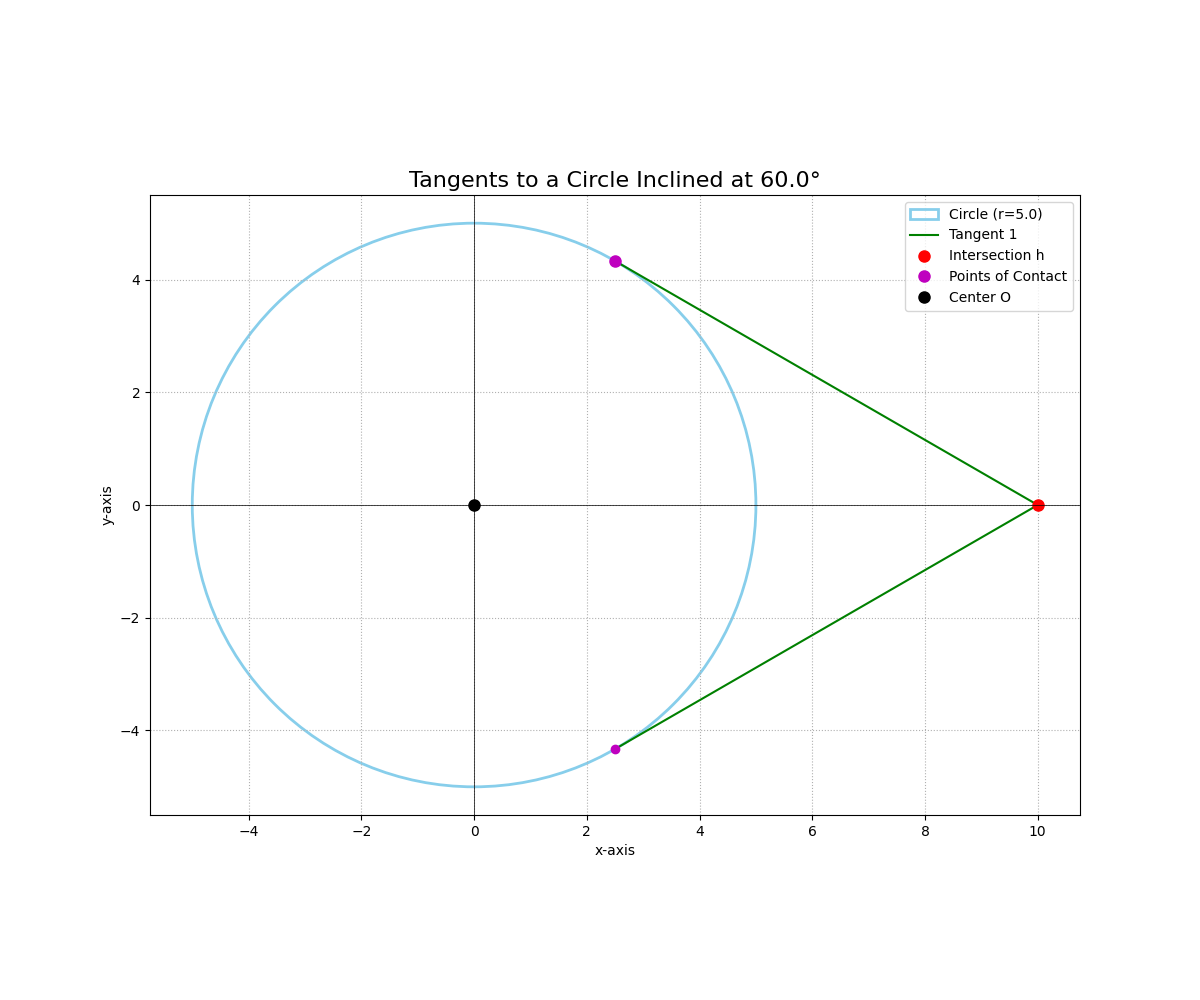
\includegraphics[width=0.65\columnwidth]{figs/1.png}
\end{figure}
\end{frame}
\end{document}
